\section{Osnovni algoritmi pretrage}

Jedan od osnovnih problema pretrage stringova je problem nala\v zenja svih pojavljivanja jednog stringa u drugom. Formalno, za data dva stringa $s,p$ du\v zina $n$ i $m$, redom, na\' ci sve indekse $i$ takve da je $0 \leq i \leq n-m$ i $s_{[i, i+m)} = p$. String $s$ unutar kojeg se tra\v zi se \v cesto naziva tekstom, dok se $p$ naziva re\v cju (iako ne mora biti jedna re\v c) ili \textit{pattern}-om odnosno \v sablonom. U literaturi na engleskom jeziku se \v cesto sre\' cu i pojmovi \textit{haystack} (plast sena) i \textit{needle} (igla).

\subsection{Naivna pretraga}

Naivna pretraga re\v sava prethodno opisani problem tako \v sto za svako celo $i$ iz segmenta $[0,n-m]$ upore\dj uje karakter po karakter stringove $s_{[i, i+m)}$ i $p$, pri \v cemu se odmah zaustavlja ukoliko nai\dj e na dva razli\v cita karaktera. Ovo pore\dj enje ima vremensku slo\v zenost $O(m)$ pa ceo algoritam ima vremensku slo\v zenost $O((n-m)m)$, ova slo\v zenost se dosti\v ze npr. za stringove koji se sastoje samo od slova \texttt{a}.

\lstinputlisting[language=C++, title={\textit{Implementacija naivne pretrage}}, style=customcpp]{cpp/naivna.cpp}

\subsection{Knuth-Morris-Pratt algoritam}

KMP je prvi otkriveni algoritam koji re\v sava problem pretrage stringa u linearnom vremenu, odnosno u slo\v zenosti $O(n+m)$.\cite{kmprad} Da bismo razumeli rad algoritma, defini\v simo slede\' ce pojmove.

\begin{dfn}
Sufiks-prefiks nepraznog stringa $s$ je svaki string $p$ razli\v cit od $s$, uklju\v cuju\' ci i prazan string, koji je istovremeno i sufiks i prefiks stringa $s$, tj. $s_{[0, |p|)} = s_{[|s|-|p|, |s|)} = p$.
\end{dfn}

Ozna\v cimo sa $g(s)$ du\v zinu najdu\v zeg sufiks-prefiksa stringa $s$. Za prazan string $s$ defini\v semo $g(s) = -1$. Ova funkcija zadovoljava slede\' cu, va\v znu osobinu:

\begin{thm}
\label{sufiksprefiksteorema}
Neka je $s$ neprazan string. Neka je $s' = s_{[0, |s|-1)}$, tada je $g(s) \leq g(s') + 1$.
\end{thm}

\textit{Dokaz.} Pretpostavimo suprotno, da je $g(s) > g(s') + 1$. Neka je $p$ najdu\v zi sufiks prefiks stringa $s$. Neka je $p' = p_{[0, |p|-1)}$. Tada je $p'$ sufiks-prefiks stringa $s'$, pa je $g(s') \geq |p'| = |p| - 1 = g(s) - 1$, kontradikcija. \hfill $\square$

Ukoliko je $p$ najdu\v zi sufiks-prefiks stringa $s$, tada je i svaki drugi sufiks-prefiks stringa $s$ ujedno i sufiks-prefiks stringa $p$. Ova osobina nam omogu\' cava da opi\v semo sve sufiks-prefikse nekog stringa $s$ kao lanac, gde je svaki naredni string najdu\v zi sufiks-prefiks prethodnog, sve dok se ne do\dj e do praznog stringa.

\begin{dfn}
Niz neuspeha stringa $s$ je niz $f_0, f_1, \ldots, f_{|s|}$, gde je $f_i = g(s_{[0, i)})$.
\end{dfn}

Prvi korak KMP algoritma je nala\v zenje niza neuspeha za string $p$. Prvo upisujemo $f_0 = -1$. Zatim, za svako $i > 0$, tra\v zimo najdu\v zi sufiks-prefiks stringa $p_{[0, i-1)}$ koji se mo\v ze pro\v siriti slovom $p_{i-1}$, odnosno, nalazimo najve\' ci broj $r$ takav da je $r$ du\v zina nekog sufiks-prefiksa stringa $p_{[0, i-1)}$ i va\v zi $p_r = p_{i-1}$. Ukoliko ne na\dj emo takav broj $r$, onda je $f_i = 0$. U suprotnom, po\v sto je $p_{[0, r)} = p_{[i-1-r, i-1)}$ i $p_r = p_{i-1}$ imamo da je $p_{[0, r+1)} = p_{[i-r-1, i)}$, odnosno, $r+1$ je du\v zina jednog sufiks-prefiksa stringa $p_{[0, i)}$. Iz prethodnog razmatranja imamo da je ovo upravo najdu\v zi sufiks-prefiks stringa $p_{[0,i)}$, pa upisujemo $f_i = r+1$. Niz svih sufiks-prefiksa mo\v zemo na\' ci primenom opisane osobine lanca i \v cinjenice da smo u $i$-tom koraku ve\' c izra\v cunali du\v zine najdu\v zih sufiks-prefiksa za sve prefikse stringa $p$ du\v zine manje od $i$.

\noindent \textbf{Primer.} Posmatrajmo string \texttt{atamatata}. Njegov niz neuspeha dat je u slede\' coj tabeli. Indeksi u donjem redu su pomereni za jedno mesto da bi se bolje videlo o kom prefiksu je re\v c.
\begin{center}
\begin{tabular}{|c|c|c|c|c|c|c|c|c|c|}
    \hline
    & a & t & a & m & a & t & a & t & a \\
    \hline
 -1 & 0 & 0 & 1 & 0 & 1 & 2 & 3 & 2 & 3 \\
    \hline
\end{tabular}
\end{center}

Posmatrajmo \v sta se de\v sava pri ra\v cunanju $f_i$ za pretposlednji prefiks, du\v zine $8$. U prethodnom koraku smo imali string \texttt{atamata}, kome je najdu\v zi sufiks-prefiks string \texttt{ata}. Ako poku\v samo da dodamo na njega slovo \texttt{t}, ne\' cemo dobiti poklapanje jer je na poziciji $3$ slovo \texttt{m}, zato poku\v savamo sa narednim sufiks-prefiksom odnosno $r = f_3 = 1$. Sada uspe\v sno dodajemo slovo \texttt{t} i upisujemo $r+1 = 2$ u $f_8$.

\lstinputlisting[language=C++, title={\textit{Implementacija nala\v zenja niza neuspeha kod KMP algoritma}}, style=customcpp]{cpp/kmp-ff.cpp}

Ocenimo slo\v zenost ovog algoritma. Jasno je da slo\v zenost srazmerna zbiru broja iteracija ove dve petlje. Posmatrajmo vrednost $2i-r$. Nakon svake iteracije \textit{while} petlje imamo da se $r$ smanjuje, jer je $f_r < r$ pa se $2i-r$ pove\' cava. U jednoj iteraciji \textit{for} petlje imamo da se i $i$ i $r$ pove\' cavaju za ta\v cno $1$, pa se $2i-r$ ponovo pove\' cava. Kako je po\v cetna vrednost $2i-r$ jednaka $3$, a va\v zi $2i-r \leq 2m+1$, ukupan broj iteracija, a samim tim i slo\v zenost algoritma je $O(m)$.

Opi\v simo sada glavni algoritam za tra\v zenje stringa. Algoritam za svaki prefiks $i$ stringa $s$ nalazi najdu\v zi sufiks koji je ujedno i prefiks stringa $p$. Ukoliko je du\v zina tog prefiksa jednaka $|p|$, tada dolazi do poklapanja na poziciji $i-|p|$. Neka je ta du\v zina jednaka $r_i$. Za $i=0$ imamo $r_0 = 0$. Za svako $i>0$, kre\' cemo od prefiksa stringa $p$ du\v zine $r_{i-1}$ i proveravamo da li je naredno slovo jednako slovu $s_{i-1}$. Ako jeste, zaustavljamo se i upisujemo du\v zinu na\dj enog prefiksa u $r_i$, u suprotnom, slede\' ci prefiks koji poku\v savamo da produ\v zimo je prefiks du\v zine $f_{r_{i-1}}$. Ovaj postupak ponavljamo sve dok ne do\dj emo do poklapanja ili do fiktivnog prefiksa $-1$, u tom slu\v caju du\v zina poklapanja je $0$. Primetimo da je ovaj deo algoritma veoma sli\v can nala\v zenju niza neuspeha.

\lstinputlisting[language=C++, title={\textit{Implementacija glavnog dela KMP algoritma}}, style=customcpp]{cpp/kmp-main.cpp}

Na potpuno isti na\v cin se ocenjuje slo\v zenost glavnog dela algoritma, posmatranjem vrednosti izraza $2i-r$. Slo\v zenost je $O(n+m)$, zajedno sa prvom fazom, ukupna slo\v zenost je tako\dj e $O(n+m)$.

Cela implementacija algoritma se mo\v ze zna\v cajno pojednostaviti na slede\' ci na\v cin: Posmatrajmo string $p\$s$, gde je $\$$ karakter koji se ne javlja u stringovima $p,s$. Na osnovu njegovog niza neuspeha mo\v zemo da zaklju\v cimo gde se sve pojavljuje $p$ u $s$, ta\v cnije, $i$ je pojavljivanje $p$ u $s$ akko je $f_{i+2m+1} = m$.

\noindent
\begin{minipage}[l]{\textwidth}
\lstinputlisting[language=C++, title={\textit{Pojednostavljena implementacija celog algoritma}}, style=customcpp]{cpp/kmp-simple.cpp}
\end{minipage}

\subsection{Z-algoritam}

Osnovna ideja ovog algoritma je da se izra\v cuna Z-niz, koji se defini\v se na slede\' ci na\v cin.

\begin{dfn}
Za string $s$ du\v zine $n$, Z-niz je niz $z_1, \ldots, z_{n-1}$ gde je $z_i$ du\v zina najdu\v zeg zajedni\v ckog prefiksa za stringove $s$ i $s_{[i, n)}$.
\end{dfn}

Z-niz se mo\v ze iskoristiti za pretragu stringova. Ukoliko na\dj emo Z-niz za string $ps$, $i$ je pojavljivanje $p$ u $s$ akko je $z_{i+m} \geq m$.

Z-algoritam je efikasan algoritam za nala\v zenje Z-niza.\cite{zalgoknjiga} Ozna\v cimo sa $q$ string za koji nalazimo Z-niz. Klju\v cna ideja je da se prethodno izra\v cunate vrednosti Z-niza mogu iskoristiti da se postavi bolja po\v cetna vrednost za $z_i$, umesto da se svaki put kre\' ce od nule. Naime, neka je $[l,r)$ prozor koji odgovara onom do sada na\dj enom poklapanju sa prefiksom stringa $s$ kod kojeg je $r$ najve\' ce. Drugim re\v cima, $r$ je najve\' ca na\dj ena vrednost izraza $j+z_j$ za $j<i$, a pritom je $l = j$ za koje se dosti\v ze taj maksimum. Ukoliko va\v zi $l \leq i < r$, tada znamo da je $q_{[i, r)} = q_{[i-l, r-l)}$. Tako\dj e, va\v zi $q_{[i-l, i-l+z_{i-l})} = q_{[0, z_{i-l})}$ pa, ako ozna\v cimo sa $z'_i = \min(z_{i-l}, r-i)$, va\v zi $q_{[i, i+z'_i)} = q_{[0, z'_i)}$ odnosno $z_i \geq z'_i$. Algoritam postavlja po\v cetnu vrednost $z_i = z'_i$. Zatim, dokle god se slova na pozicijama $z_i$ i $i + z_i$ poklapaju i nije dostignut kraj stringa, $z_i$ se pove\' cava za $1$.

\noindent
\begin{minipage}[l]{\textwidth}
\lstinputlisting[language=C++, title={\textit{Implementacija Z-algoritma za pretragu stringa}}, style=customcpp]{cpp/z-algo.cpp}
\end{minipage}

\noindent \textbf{Primer.} Posmatrajmo string \texttt{anananakananas}, i neka je $i=10$, odnosno, treba da izra\v cunamo vrednost $z_{10}$ tj. najdu\v zi zajedni\v cki prefiks stringova \texttt{anananakananas} i \texttt{anas}. Od svih prozora kojima je levi kraj $l < i$, najve\' ce $r$ ima $[l,r) = [8,13)$.

\begin{figure}[H]
    \centering
    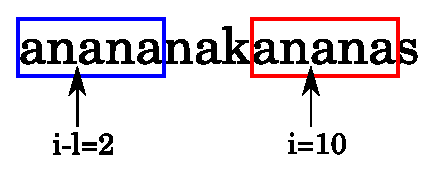
\includegraphics[width=40mm]{../img/zalgo1.eps}
    \caption*{\textit{Ilustracija prozora kod Z-algoritma}}
\end{figure}

Na osnovu toga \v sto je $s_{[8,13)} = s_{[0,5)}$ prozor imamo da je podstring $s_{[10,13)}$ jednak podstringu $s_{[2,5)}$. Vrednost $z_2$ je jednaka $5$, pa va\v zi da je $s_{[2,7)} = s_{[0,5)}$. Iz druge jednakosti mo\v zemo zaklju\v citi da je $s_{[0,3)} = s_{[2,5)}$, a iz prve da je $s_{[2,5)} = s_{[10,13)}$, pa postavljamo po\v cetnu vrednost $z_{10}$ na $3$. Kako je $s_{13}$ slovo $s$, a $s_3$ slovo $n$, odmah se zaustavljamo, vrednost $z_{10}$ je jednaka $3$.

Doka\v zimo da ovaj algoritam ima slo\v zenost $O(n+m)$. O\v cigledno, kriti\v cna je unutra\v snja \textit{while} petlja. Dokaza\' cemo da svaka iteracija \textit{while} petlje odgovara pove\' canju vrednosti promenljive $r$ za bar $1$. Posmatrajmo slede\' ce slu\v cajeve:

\begin{itemize}
\item Pre ulaska u \textit{while} petlju va\v zi $i \geq r$. U ovom slu\v caju $z_i$ ima po\v cetnu vrednost nula, na kraju \textit{while} petlje \' ce va\v ziti $i + z_i \geq r$ pa \' ce $r$ dobiti vrednost $i + z_i$, odnosno $r$ \' ce se pove\' cati za barem $z_i$, \v sto je ve\'ce ili jednako od broja iteracija \textit{while} petlje.
\item Pre ulaska u \textit{while} petlju va\v zi $i < r$ i $z_{i-l} < r-i$. Sada $z_i$ dobija po\v cetnu vrednost $z_{i-l}$. Doka\v zimo da \' ce \textit{while} petlja izvr\v siti ta\v cno nula iteracija. Pretpostavimo suprotno, da je $q_{i+z_i} = q_{z_i}$, odnosno $q_{i+z_{i-l}} = q_{z_{i-l}}$. Iz definicije prozora $[l, r)$ imamo da je $q_{[0, r-l)} = q_{[l, r)}$, po\v sto je $l \leq i+z_{i-l} < r$, odnosno, ova pozicija je unutar prozora, va\v zi $q_{i+z_{i-l}} = q_{i-l+z_{i-l}}$, odnosno, po pretpostavci, $q_{z_{i-l}} = q_{i-l+z_{i-l}}$, \v sto zna\v ci da $z_{i-l}$ ima pogre\v sno izra\v cunatu vrednost jer se poklapaju karakteri na kraju odgovaraju\' cih podstringova, \v sto dovodi do kontradikcije.
\item Pre ulaska u \textit{while} petlju va\v zi $i < r$ i $z_{i-l} \geq r-i$. Sada $z_i$ dobija po\v cetnu vrednost $r-i$. Ako petlja izvr\v si $k$ iteracija, na kraju \' ce va\v ziti $z_i=k+r-i$ odnosno $i+z_i=k+r$, \v sto zna\v ci da \' ce nova vrednost $r$ biti za bar $k$ ve\' ca.
\end{itemize}

Kako je $r \leq n+m$ zaklju\v cujemo da je ukupna slo\v zenost $O(n+m)$.
